\newcommand{\psd}[1]{{\small\sffamily{\color{blue!60}#1}}}


\subsection{Parallel 2D tensile cracking and calculate-ploting reaction-force}

In solid mechanics often the quantities of interest includes plots such
as reaction-force on a surface vs.~the applied force. Often times these
are experimental outputs and are used for validation.

PSD provides routines to calculate the reaction force on a surface and
also provides means of live plotting (run-time) of these results.
Imagine the test case of tensile cracking of plate (2D) as discussed
above. Considering we are now interested in seeing the plot of reaction
force at surface vs.~the applied tensile displacement, we would need to
use two extra flags in the \psd{ PSD\_PreProcess} step. These flags are
\psd{-getreactionforce} and \psd{ -reactionforce  stress\_based } as
read below:

\begin{lstlisting}[style=BashInputStyle]
PSD_PreProcess -dimension 2 -problem damage -model hybrid_phase_field \
-dirichletconditions 2 -getreactionforce -reactionforce stress_based
\end{lstlisting}

The flag \psd{-getreactionforce} directs PSD to include the routines to
get the reaction force and \psd{ -reactionforce  stress\_based } is the
method by which we get reaction force, in this case reaction force is
calculated using integral of stress in \(y\) direction
\(F_y=\int_{\partial\Omega_{top}} \sigma_y\). Other method
\psd{ -reactionforce variational\_based} also exists within PSD, which
is more accurate but slower, this method calculates reaction force based
on matrix vector multiplication \({F_x,F_y}=\mathbf{A}{u_1,u_2}\) .

Run the problem in the usual way bu using \psd{ PSD\_Solve} and
appropriate number of processes and mesh. While the PSD solver runs it
will create a file \psd{ force.data} that contains the reaction force
and the applied traction.

\begin{lstlisting}[style=BashInputStyle]
PSD_Solve -np 4 Main.edp -mesh ./../Meshes/2D/tensile-crack.msh -v 0
\end{lstlisting}

You can then go ahead and plot \psd{ force.data} to see how \(F_y\) and
\(F_x\) evolve with \(\Delta u_2\). Within the file the first column is
the loading \(\Delta u_2\), the second and the third columns are the
forces \(F_x\) and \(F_y\).

\begin{figure}[h!]
\centering

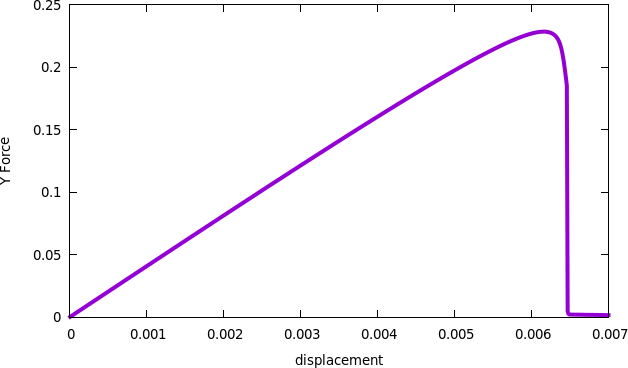
\includegraphics[width=0.4\textwidth]{./Images/plot-fd.png}
\caption{Applied traction vs. force in y direction. \label{fd-plot}}
\end{figure}

Optionally if you have GnuPlot configured with PSD you can see live
ploting of this curve if you use option \psd{-plotreactionforce} during
the \psd{ PSD\_PreProcess}.

\begin{figure}[h!]
\centering

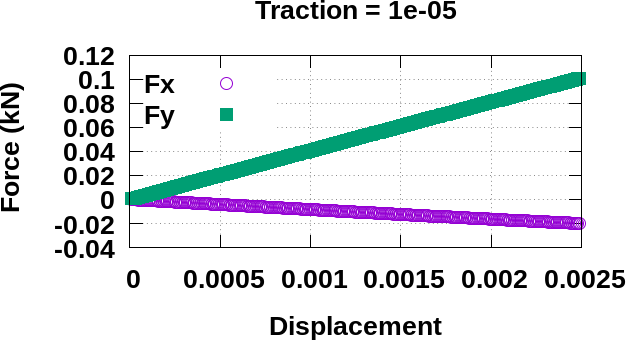
\includegraphics[width=0.3\textwidth]{./Images/gp0.png}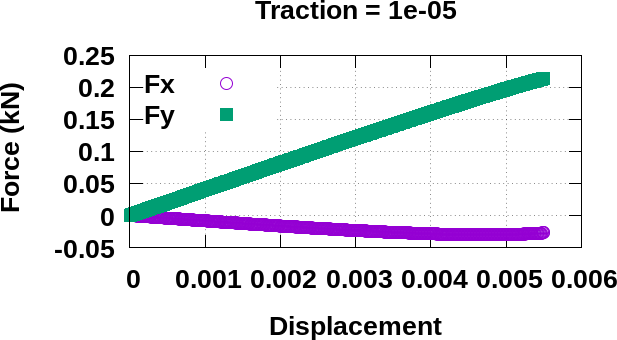
\includegraphics[width=0.3\textwidth]{./Images/gp1.png}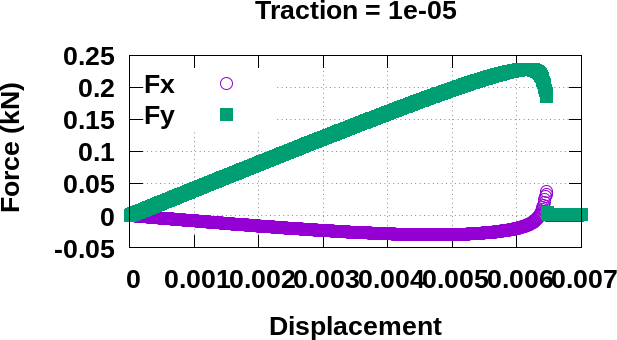
\includegraphics[width=0.3\textwidth]{./Images/gp2.png}
\caption{Applied traction vs. force in y direction plotted live using PSD. \label{gnuplot-plot}}
\end{figure}

\textbf{Parallel 3D and calculate reactionforce}

\begin{lstlisting}[style=BashInputStyle]
PSD_PreProcess -dimension 3 -problem damage -model hybrid_phase_field \
-dirichletconditions 2 -getreactionforce -reactionforce stress_based
\end{lstlisting}

\begin{lstlisting}[style=BashInputStyle]
PSD_Solve -np 3 Main.edp -mesh ./../Meshes/3D/tensile-crack.msh -v 0
\end{lstlisting}
